\documentclass[11pt]{article}
\usepackage[scaled=0.92]{helvet}
\usepackage{geometry}
\geometry{letterpaper,tmargin=1in,bmargin=1in,lmargin=1in,rmargin=1in}
\usepackage[parfill]{parskip} % Activate to begin paragraphs with an empty line rather than an indent %\usepackage{graphicx}
\usepackage{amsmath,amssymb, mathrsfs,  mathtools, dsfont}
\usepackage{tabularx}
\usepackage{tikz-cd}
\usepackage[font=footnotesize,labelfont=bf]{caption}
\usepackage{graphicx}
\usepackage{xcolor}
%\usepackage[linkbordercolor ={1 1 1} ]{hyperref}
%\usepackage[sf]{titlesec}
\usepackage{natbib}
\usepackage{../../Tianpei_Report}

%\usepackage{appendix}
%\usepackage{algorithm}
%\usepackage{algorithmic}

%\renewcommand{\algorithmicrequire}{\textbf{Input:}}
%\renewcommand{\algorithmicensure}{\textbf{Output:}}



\begin{document}
\title{Lecture 2: Connectedness and Compactness}
\author{ Tianpei Xie}
\date{Nov. 7th., 2022}
\maketitle
\tableofcontents
\newpage
\section{Connected Spaces}
\subsection{Definitions}
\begin{itemize}
\item \begin{definition}(\emph{\textbf{Separation} and \textbf{Connectedness}})\\
Let $X$ be a topological space. A \emph{\textbf{separation}} of $X$ is a pair $U$, $V$ of \emph{\textbf{disjoint} nonempty \textbf{open} subset}s of $X$ whose union is $X$. 

The space $X$ is said to be \underline{\emph{\textbf{connected}}} if there \emph{does not exist a separation} of $X$.
\end{definition}

\item  \begin{definition} (\emph{\textbf{Connected: Equivalent Definition}})\\
Equivalently, $X$ is \emph{\textbf{connected}} if and only if the only subsets of $X$ that are \emph{\textbf{both open and closed}} are $\emptyset$
and $X$ itself.
\end{definition}

\item \begin{remark} (\emph{\textbf{Proof of Connectedness}})\\
As the definition suggests, the proof of connectedness is done \emph{\textbf{by contradition}}. One first assume that the set $X$ has a \emph{\textbf{seperation}}; it can be separated into two \emph{\textbf{disjoint nonempty open}} sets such that $X = A \cup B$. Then we proof by contradiction using \emph{\textbf{existing connectedness conditions}} and the \emph{\textbf{property of open subsets (basis, continuity etc.)}}.
\end{remark}

\item \begin{remark}
\emph{\textbf{Connectedness}} is obviously a \emph{\textbf{topological property}}, since it is formulated entirely in terms of \emph{the collection of open sets} of $X$. 

Said differently, if $X$ is \emph{\textbf{connected}}, so is any space \emph{\textbf{homeomorphic}} to $X$.
\end{remark}

\item \begin{lemma}(\textbf{Separation and Connected Subspace}) \citep{munkres2000topology}\\
If $Y$ is a \textbf{subspace} of $X$, a \textbf{separation} of $Y$ is a pair of disjoint nonempty sets $A$ and $B$ whose union is $Y$, \textbf{neither} of which contains a \textbf{limit point} of the other. The space $Y$ is connected if there exists no separation of $Y$.
\end{lemma}

\item \begin{example} (\emph{\textbf{Indiscrete Topology is Connected}})\\
Let $X$ denote a two-point space in \emph{\textbf{the indiscrete topology}}. Obviously there is \emph{no separation} of $X$, so $X$ is \emph{connected}.
\end{example}

\item \begin{example} (\emph{\textbf{$\bQ$ is Not Connected}})\\
The \emph{rationals} $\bQ$ are \emph{\textbf{not connected}}. Indeed, \emph{the only connected subspaces} of $\bQ$ are the \emph{one-point sets}: If $Y$ is a subspace of $\bQ$ containing two points $p$ and $q$, one can choose \emph{an irrational number} $a$ lying between $p$ and $q$, and write $Y$ as the union of the open
sets
\begin{align*}
Y \cap (-\infty, a)\text{ and }Y \cap (a, +\infty).
\end{align*}
\end{example}

\item \begin{lemma}
If the sets $C$ and $D$ form a \textbf{separation} of $X$, and if $Y$ is a \textbf{connected} subspace of $X$, then $Y$ lies \textbf{entirely within} either $C$ or $D$.
\end{lemma}

\item \begin{proposition} (\textbf{Connectedness by Union}) \citep{munkres2000topology}\\
The \textbf{union} of a collection of connected subspaces of X that \textbf{have a point in common} is connected.
\end{proposition}

\item \begin{proposition} (\textbf{Connectedness by Closure})\citep{munkres2000topology} \\
Let $A$ be a connected subspace of $X$. If $A \subseteq B \subseteq  \bar{A}$, then $B$ is also connected.
\end{proposition}

\item \begin{remark}
If $B$ is formed by \emph{adjoining} to the \emph{\textbf{connected} subspace $A$ some or all of its \textbf{limit points}}, then $B$ is connected.
\end{remark}

\item \begin{proposition}  (\textbf{Connectedness by Continuity}) \citep{munkres2000topology} \\
The \textbf{image} of a connected space under a \textbf{continuous} map is connected.
\end{proposition}

\item \begin{proposition}  (\textbf{Connectedness by Finite Product}) \citep{munkres2000topology} \\
A \textbf{finite} cartesian product of connected spaces is connected.
\end{proposition}

\item \begin{remark}
Countable infinite product of connected spaces \emph{\textbf{may not be connected}}. It depends on the \emph{\textbf{topology}} of the product space.
\end{remark}

\item \begin{example} (\emph{\textbf{$\bR^{\omega}$ is Not Connected under Box Topology}})\\
Consider the cartesian product $\bR^{\omega}$ in \emph{\textbf{the box topology}}. We can write $\bR^{\omega}$ as the union of the set $A$ consisting of \emph{all \textbf{bounded} sequences of real numbers}, and the set $B$ of \emph{all \textbf{unbounded} sequences}. These sets are \emph{\textbf{disjoint}}, and each is \emph{\textbf{open}} in the box topology.

For if $a = (a_1, a_2, \ldots)$ is a point of $\bR^{\omega}$, the open set
\begin{align*}
U = (a_1 - 1, a_1 + 1) \times (a_2 - 1, a_2 + 1) \times \ldots
\end{align*}
consists \textbf{\emph{entirely}} of \textbf{\emph{bounded}} sequences if $a$ is \emph{\textbf{bounded}}, and of \emph{unbounded sequences} if $a$ is \emph{unbounded}. Thus, even though $\bR$ is \emph{connected} (as we shall prove in the next section),  $\bR^{\omega}$ is \emph{not connected in the box topology}. \qed
\end{example}

\item \begin{example} (\emph{\textbf{$\bR^{\omega}$ is  Connected under Product Topology}})\\
Consider the cartesian product $\bR^{\omega}$ in \emph{\textbf{the product topology}}. Let $\widetilde{\bR}^n$ denote the \emph{\textbf{subspace}} of $\bR^{\omega}$ consisting of all sequences $x = (x_1, x_2, \ldots)$ such that $x_i = 0$ for $i > n$. The space $\widetilde{\bR}^n$  is clearly
\emph{\textbf{homeomorphic}} to $\bR^n$, so that it is \emph{\textbf{connected}}. It follows that the space $\bR^{\infty}$ that is the \emph{\textbf{union}} of the spaces $\widetilde{\bR}^n$ is \emph{\textbf{connected}}, for these spaces have the point $0 = (0, 0, \ldots)$ in common.  We show that the \emph{\textbf{closure}} of $\bR^{\infty}$ equals all of $\bR^{\omega}$, from which it follows that $\bR^{\omega}$ is \emph{\textbf{connected}} as well. 

Let $a = (a_1, a_2, \ldots)$ be a point of $\bR^{\omega}$. Let $U = \prod_i U_i$ be a \emph{\textbf{basis}} element for the product topology that contains $a$. We show that $U$ \emph{\textbf{intersects}} $\bR^{\infty}$. There is an integer $N$ such that $U_i = \bR$ for $i > N$. Then the point
\begin{align*}
x = (a_1 \xdotx{,} a_n, 0, 0, \ldots)
\end{align*}
of $\bR^{\omega}$ belongs to $U$, since $a_i \in U_i$ for all $i$, and $0 \in U_i$ for $i > N$. \qed
\end{example}
\end{itemize}


\subsection{Connected Subspaces of the Real Line}
\begin{itemize}
\item \begin{definition}(\textbf{\emph{Linear Continuum}}) \\
A \emph{\textbf{simply ordered set}} $L$ having \emph{more than one element} is called a \underline{\emph{\textbf{linear continuum}}} if the following hold:
\begin{enumerate}
\item $L$ has the \emph{\textbf{least upper bound property}}.
\item If $x < y$, there exists $z$ such that $x < z < y$.
\end{enumerate}
\end{definition}

\item \begin{proposition} (\textbf{Linear Continuum is Connected}) \citep{munkres2000topology} \\
If $L$ is a \textbf{linear continuum} in the \textbf{order topology}, then $L$ is \textbf{connected}, and so are \textbf{intervals} and \textbf{rays} in $L$.
\end{proposition}
\begin{proof}
Recall that a subspace $Y$ of $L$ is said to be \emph{\textbf{convex}} if for every pair of points $a$, $b$ of $Y$ with $a < b$, the entire interval $[a, b]$ of points of $L$ lies in $Y$. We prove that if $Y$ is a \emph{\textbf{convex subspace}} of $L$, then $Y$ is \emph{\textbf{connected}} ($L$ itself is \emph{convex}).

So suppose that $Y$ is the union of the disjoint nonempty sets $A$ and $B$, each of which is \textit{\textbf{open}} in $Y$. Choose $a \in A$ and $b \in B$; suppose for convenience that $a < b$. The interval $[a, b]$ of points of $L$ is contained in $Y$. Hence $[a, b]$ is the union of the disjoint sets
\begin{align*}
A_0 = A \cap [a, b]\text{ and }B_0 = B \cap [a, b],
\end{align*}
each of which is \emph{open} in $[a, b]$ in the \emph{subspace topology}, which is the same as the \emph{order topology}. The sets $A_0$ and $B_0$ are \emph{nonempty} because $a \in A_0$ and $b \in B_0$. Thus, $A_0$ and $B_0$ constitute a \emph{\textbf{separation}} of $[a, b]$. 

Let $c = \sup A_0$ is \emph{\textbf{the least upper bound}} of $A_0$. We show that $c$ belongs \emph{\textbf{neither}} to $A_0$ nor to $B_0$, which contradicts
the fact that $[a, b]$ is the \emph{union} of $A_0$ and $B_0$.
\begin{enumerate}
\item Suppose that $c \in B_0$. Then $c \neq a$, so either $c = b$ or $a < c < b$. In either case, it follows from the fact that $B_0$ is \emph{\textbf{open}} in $[a, b]$ that there is \emph{some interval} of the form $(d, c]$ \emph{contained} in $B_0$. If $c = b$, we have a contradiction at once, for $d$ is a \emph{\textbf{smaller upper bound}} on $A_0$ \emph{than} $c$. (To prove $d > x$ for any $x \in A_0$, we assume that there exists some $x_0 \in A_0$ such that $d < x_0$. However, the interval $(d, x_0)\subset (d, b]$ belongs to $B_0$, contradiction.)

If $c < b$, we note that $(c, b]$ does not intersect $A_0$ (because $c$ is an upper bound on $A_0$). Then
\begin{align*}
(d, b] = (d, c] \cup (c, b]
\end{align*}
does not intersect $A_0$. Again, $d$ is a \emph{\textbf{smaller upper bound}} on $A_0$ than $c$, contrary to construction. 

\item Suppose that $c \in A_0$. Then $c \neq b$, so either $c = a$ or $a < c < b$. Because $A_0$ is open in $[a, b]$, there must be some interval of the form $[c, e)$ contained in $A_0$. Because of \emph{order property (2)} of \emph{\textbf{the linear continuum}} $L$, we can choose a point $z$ of $L$ such that $c < z < e$. Then $z \in A_0$, contrary to the fact that $c$ is \emph{an upper bound} for $A_0$. \qed
\end{enumerate}
\end{proof}

\item \begin{corollary} (\textbf{$\bR$ is Connected})\\
The real line $\bR$ is \textbf{connected} and so are \textbf{intervals} and \textbf{rays} in $\bR$.
\end{corollary}

\item \begin{theorem} (\textbf{Intermediate Value Theorem}).  \citep{munkres2000topology}\\
Let $f : X \rightarrow Y$ be a \textbf{continuous} map, where $X$ is a \textbf{connected} space and $Y$ is an ordered set in the \textbf{order topology}. If $a$ and $b$ are two points of $X$ and if $r$ is a point of $Y$ lying between $f(a)$ and $f(b)$, then there \textbf{exists} a point $c$ of X such that $f(c) = r$.
\end{theorem}
\begin{proof}
Assume the hypotheses of the theorem. The sets
\begin{align*}
A = f(X) \cap (-\infty, r)\text{ and }B = f(X) \cap (r, +\infty)
\end{align*}
are \emph{disjoint}, and they are \emph{nonempty} because one contains $f(a)$ and the other contains $f(b)$. Each is \emph{open} in $f(X)$, being the \emph{intersection} of an open ray in $Y$ with $f(X)$. 

If there were no point $c$ of $X$ such that $f(c) = r$, then $f(X)$ would be the \emph{union} of the
sets $A$ and $B$. Then $A$ and $B$ would constitute a separation of $f(X)$, contradicting the fact that \emph{the image of a connected space under a continuous map} is \emph{connected}. \qed
\end{proof}

\item \begin{definition} (\emph{\textbf{Path Connectedness}})\\
Given points $x$ and $y$ of the space $X$, a \underline{\emph{\textbf{path}}} in $X$ from $x$ to $y$ is a \emph{continuous map} $f : [a, b] \rightarrow X$ of some \emph{\textbf{closed interval}} in the real line into $X$, such that $f(a) = x$ and $f(b) = y$. 

A space $X$ is said to be \underline{\emph{\textbf{path connected}}} if \emph{\textbf{every pair}} of points of $X$ can be \emph{\textbf{joined by a path}} in $X$.
\end{definition}

\item \begin{remark}
It is easy to see that \emph{\textbf{a path-connected space $X$ is connected}} since $X = f([a,b])$ is the image of connected space under continuous function $f$. The \emph{converse} is \emph{not true}, i.e. connected $\not\Rightarrow$ path-connected.
\end{remark}


\item \begin{example} (\emph{\textbf{Punctured Euclidean Space $\bR^n \setminus \set{0}$ is Path Connected}})\\
Define \emph{\textbf{punctured euclidean space}} to be the space $\bR^n \setminus \set{0}$, where $0$ is the origin in $\bR^n$. If $n > 1$, this space is \emph{\textbf{path connected}}: Given $x$ and $y$ different from $0$, we can join $x$ and $y$ by the \emph{straight-line path} between them if that path does not go through
the origin. Otherwise, we can choose a point $z$ \emph{not on the line joining $x$ and $y$}, and take the \emph{broken-line path} from $x$ to $z$, and then from $z$ to $y$.
\end{example}

\item 
\begin{example} (\emph{Common Path-Connected Spaces})\\
The following spaces are \emph{\textbf{path-connected}}:
\begin{enumerate}
\item \emph{\textbf{The unit ball}} $\bB^n = \set{x: \norm{x}{} \le 1}$ is \emph{path-connected};
\item \emph{\textbf{The unit sphere}} $\bS^{n-1}$ in $\bR^n$ by the equation $\bS^{n-1} = \set{x: \norm{x}{} = 1}$ is \emph{path connected}. For the map $g : \bR^n \setminus \set{0}\rightarrow \bS^{n-1}$ defined by $g(x)= x/\norm{x}{}$ is \textit{continuous} and \emph{surjective}; and the continuous image of path connected space is path connected.
\end{enumerate}
\end{example}

\begin{figure}
\begin{minipage}[t]{1\linewidth}
  \centering
  \centerline{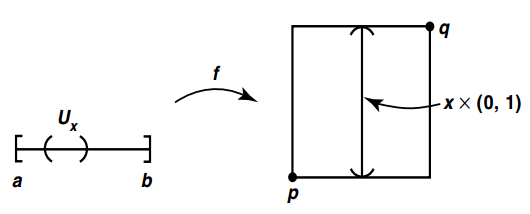
\includegraphics[scale = 0.5]{order_square_not_path_connected.png}}
\end{minipage}
\caption{\footnotesize{\textbf{The proof that ordered square is not path connected. \citep{munkres2000topology}}}}
\label{fig: order_square_not_path_connected}
\end{figure}



\item \begin{example}
\emph{\textbf{The ordered square}} $I_o^2$ is \emph{\textbf{connected}} but \emph{\textbf{not path connected}}.
\end{example}
\begin{proof}
Being a linear continuum, \emph{the ordered square} is \emph{\textbf{connected}}. Let $p = (0, 0)$ and $q =
(1,1)$. We suppose there is a path $f : [a, b] \rightarrow I_o^2$ joining $p$ and $q$ and derive a contradiction.

The image set $f([a, b])$ must contain every point $(x, y)$ of $I_o^2$, by \emph{the intermediate value theorem}. Therefore, for each $x \in I$, the set
\begin{align*}
U_x = f^{-1}(x \times (0, 1))
\end{align*}
is a \emph{nonempty subset} of $[a, b]$; by \emph{continuity}, it is \emph{\textbf{open}} in $[a, b]$. See Figure \ref{fig: order_square_not_path_connected}. Choose, for each $x \in I$, a \emph{\textbf{rational number}} $q_x$ belonging to $U_x$. Since the sets $U_x$ are \emph{disjoint}, the map $x \mapsto q_x$ is an \emph{\textbf{injective}} mapping of $I$ into $\bQ$. This contradicts the fact that the interval $I$ is \emph{\textbf{uncountable}} (which we shall prove later) \qed
\end{proof}

\begin{figure}
\begin{minipage}[t]{1\linewidth}
  \centering
  \centerline{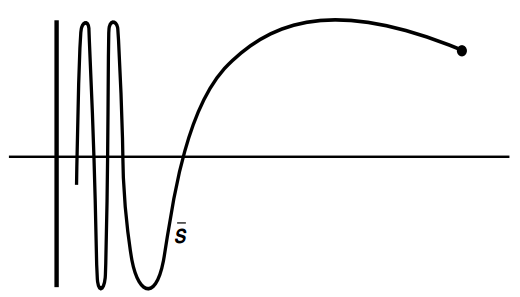
\includegraphics[scale = 0.5]{topologist_sine_curve.png}}
\end{minipage}
\caption{\footnotesize{\textbf{The topologist's sine curve is connected but not path connected. \citep{munkres2000topology}}}}
\label{fig: topologist_sine_curve}
\end{figure}


\item \begin{example} 
\emph{\textbf{The topologist's sine curve}} is defined as the \emph{\textbf{closure}} $\bar{S}$ of the set
\begin{align*}
S = \set{(x, \sin(1/x)): 0 < x \le 1}.
\end{align*} $S$ is \emph{\textbf{connected}} but \emph{\textbf{not path-connected}}.

Note that $f(t)= (x(t), y(t))$ where $x(t) = t$ and $y(t) = \sin(1/x(t))$ are both \emph{continuous}, so $f(t)$ is \emph{continuous}.  $S$ is the image of the connected set $(0, 1]$ under a continuous map $f$, so $S$ is \emph{\textbf{connected}}. Therefore, \emph{\textbf{its closure}} $\bar{S}$ in $\bR^2$ is also \emph{connected}.  From Figure \ref{fig: topologist_sine_curve}, we see that $\bar{S}$ equals the union of $S$ and the vertical interval $0 \times [-1, 1]$. We show that $\bar{S}$ is \emph{not path connected}.

Suppose there is a path $f : [a, c] \rightarrow \bar{S}$ beginning at the origin and ending at a point of $S$. The set of those $t$ for which $f(t) \in 0 \times [-1, 1]$ is \emph{\textbf{closed}}, so it has a \emph{\textbf{largest element}} $b$. Then $f : [b, c] \rightarrow \bar{S}$ is a \emph{path} that maps $b$ into the vertical interval $0 \times [-1, 1]$ and maps the other points of $[b, c]$ to points of $S$.

Replace $[b, c]$ by $[0, 1]$ for convenience; let $f(t) = (x(t), y(t))$. Then $x(0) = 0$, while  $x(t) > 0$ and $y(t) = \sin(1/x(t))$ for $t > 0$. We show there is a sequence of points $t_n \rightarrow 0$ such that $y(t_n) = (-1)^n$. Then the sequence $y(t_n)$ \emph{\textbf{does not converge}}, contradicting \emph{\textbf{continuity}} of $f$.

To find $t_n$, we proceed as follows: Given $n$, choose $u$ with $0 < u < x(1/n)$ such that $\sin(1/u) = (-1)^n$. Then use \emph{the intermediate value theorem} to find $t_n$ with $0 < t_n < 1/n$ such that $x(t_n) = u$. \qed
\end{example}
\end{itemize}


\subsection{Components and Local Connectedness}
\begin{itemize}
\item Given an arbitrary space $X$, there is a natural way to \emph{\textbf{break} it up into pieces} that are connected (or path connected). 
\begin{definition} (\emph{\textbf{Connected Component} as \textbf{Equivalence Class}})\\
Given $X$, define an \emph{equivalence relation} on $X$ by setting $x \sim y$ if there is \emph{a \textbf{connected subspace}} of $X$ containing \emph{both} $x$ and $y$. The \emph{equivalence classes} are called \underline{\emph{\textbf{the components}}} (or the \underline{\emph{\textbf{connected components}}}) of $X$.
\end{definition}

\item \begin{proposition} (\textbf{Characterization of Connected Components})\\
The components of $X$ are \textbf{connected disjoint subspaces} of $X$ whose union is $X$, such that each nonempty \textbf{connected} subspace of $X$ \textbf{intersects only one} of them.
\end{proposition}

\item \begin{definition}(\emph{\textbf{Path Component}})\\
We define another \emph{equivalence relation} on the space $X$ by defining $x \sim y$ if there is a \emph{path} in $X$ from $x$ to $y$. The \emph{equivalence classes} are called \emph{\underline{\textbf{the path components}} of $X$}.
\end{definition}

\item \begin{proposition} (\textbf{Characterization of Path Components})\\
The path components of $X$ are \textbf{path-connected disjoint subspaces} of $X$ whose union is $X$, such that each nonempty \textbf{path-connected} subspace of $X$ \textbf{intersects only one} of them.
\end{proposition}

\item \begin{example}
Each connected component of $\bQ$ in $\bR$ consists of \emph{a single point}. \emph{\textbf{None}} of the components of $\bQ$ are \emph{\textbf{open}} in $\bQ$. 
\end{example}

\item \begin{example}
The ``\emph{\textbf{topologist’s sine curve}}” $\bar{S}$ of the preceding section is a space that has \emph{\textbf{a single component}} (since it is \emph{connected}) and \emph{\textbf{two path components}}. One path component is the curve $S$ and the other is \emph{the vertical interval} $V = 0 \times [-1, 1]$. Note that $S$ is \emph{\textbf{open}} in $\bar{S}$ but \emph{\textbf{not closed}}, while $V$ is \emph{\textbf{closed}} but \emph{\textbf{not open}}.

If one forms a space from $\bar{S}$ by \emph{\textbf{deleting}} all points of $V$ having \emph{\textbf{rational second coordinate}}, one obtains a space that has \emph{\textbf{only one component}} but \emph{\textbf{uncountably many path components}}.
\end{example}

\item \begin{remark}
From the example of topologist's sine curve, we see that the \emph{connectedness does not imply the path-connectedness} since \emph{\textbf{neither} of \textbf{two path components} are \textbf{both} open and closed}. Note that the vertical line is the set of \emph{\textbf{limit points}} of the  curve $\sin(1/x)$ but not every sequence approaches to the vertical curve is convergent. 
\end{remark}

\item \begin{definition} (\emph{\textbf{Locally Connected} and \textbf{Locally Path-Connected}})\\
A space $X$ is said to be  \emph{\underline{\textbf{locally connected at $x$}}} if for every \emph{neighborhood} $U$ of $x$, there is a \emph{\textbf{connected neighborhood}} $V$ of $x$ \emph{contained} in $U$. If X is \emph{locally connected at each of its points}, it is said simply to be  \emph{\underline{\textbf{locally connected}}}. 

Similarly, a space $X$ is said to be \emph{\underline{\textbf{locally path connected at $x$}}} if for every \emph{neighborhood} $U$ of $x$, there is a \emph{\textbf{path-connected neighborhood}} $V$ of $x$ contained in$ U$. If $X$ is \emph{locally path connected at each of its points}, then it is said to be \emph{\underline{\textbf{locally path connected}}}.
\end{definition}


\item \begin{example}
See some of examples below:
\begin{enumerate}
\item The intervals and rays in $\bR$ are \emph{\textbf{both connected and locally connected}}.
\item The subspace $[−1, 0) \cup (0, 1]$ of $\bR$ is \emph{\textbf{not connected}}, but it is \emph{\textbf{locally connected}}.
\item The rationals $\bQ$ are \emph{\textbf{neither connected nor locally connected}}.
\item \emph{The topologist’s sine curve} is \emph{\textbf{connected}} but \emph{\textbf{not locally connected}}.
\end{enumerate} 
\end{example}


\item \begin{proposition} (\textbf{Characterization of Locally Connectedness}) \citep{munkres2000topology}\\
A space $X$ is locally connected \textbf{if and only if} for every \textbf{open} set $U$ of X, each \textbf{component} of $U$ is \textbf{open} in $X$.
\end{proposition}

\item \begin{proposition} (\textbf{Characterization of Locally Path-Connectedness}) \citep{munkres2000topology}\\
A space $X$ is locally path connected \textbf{if and only if} for every \textbf{open} set $U$ of X, each \textbf{path component} of $U$ is \textbf{open} in $X$.
\end{proposition}

\item \begin{proposition} (\textbf{Relationship between Components and Path Components})\\
If $X$ is a topological space, each \textbf{path component} of $X$ lies in a \textbf{component} of $X$. If $X$ is \textbf{locally path connected}, then the \textbf{components} and \textbf{the path components} of $X$ are the \textbf{same}.
\end{proposition}
\end{itemize}


\section{Compact Spaces}
\begin{remark} (\emph{\textbf{Metric Space} and \textbf{Compact Hausdorff Space}})\\
Two of the most well-behaved classes of spaces to deal with in mathematics are \emph{\textbf{the metrizable spaces}} and \emph{\textbf{the compact Hausdorff spaces}}. 
\begin{enumerate}
\item \underline{\emph{\textbf{Metrizable space $(X ,d)$}}}: 
\begin{itemize}
\item \emph{\textbf{subspace}} of \emph{metrizable} space is \emph{meterizable};
\item \emph{\textbf{compact subspace}} of \emph{metric} space is \emph{\textbf{bounded}} in that metric and is \emph{\textbf{closed}};
\item \emph{every metrizable space} is \emph{\textbf{normal}} ($T_4$);
\item \emph{\textbf{compactness}} $=$ \emph{\textbf{sequential compactness}} $=$ \emph{\textbf{limit point compactness}};
\item \emph{\textbf{sequence lemma}}: for $A \subset X$,  $x \in \bar{A}$ if and only if  there exists a squence of points in $A$ that converges to $x$.  ($\Rightarrow$ need $X$ being metric space);
\item $f$ is \emph{\textbf{continuous}} at $x$ if and only if $x_n \rightarrow x$ leads to $f(x_n) \rightarrow f(x)$ ($\Leftarrow$ part holds for metric space)
\item \emph{\textbf{unform limit theorem}}: If the \emph{range} of $f_n$ is a \emph{metric space} and $f_n$ are \emph{continuous}, then $f_n \rightarrow f$ \emph{uniformly} means that $f$ is a \emph{continuous} function. 
\item \emph{\textbf{unform continuity theorem}}: if $f$ is a \emph{countinous} map between two \emph{metric spaces}, and the domain is \emph{\textbf{compact}}, then $f$ is \emph{\textbf{uniformly continuous}}.
\end{itemize}

\item \underline{\emph{\textbf{Compact Hausdorff Space}}}:
\begin{itemize}
\item \emph{\textbf{subspace}} of \emph{compact Hausdorff space} is \emph{compact Hausdorff} if and only if it is \emph{\textbf{closed}}. 
\item \emph{\textbf{closed subspace}} of \emph{compact} space is \emph{\textbf{compact}}; 
\item \emph{\textbf{compact subspace}} of \emph{Hausdorff} space is \emph{\textbf{closed}};
\item \emph{compact Hausdorff space} $X$ is \textbf{\emph{normal}} ($T_4$), thus it is \emph{\textbf{completely regular}};
\item \emph{\textbf{arbitrary product}} of \emph{compact (Hausdorff)}  space is \emph{compact (Hausdorff)};
\item \emph{\textbf{compactness}} $\Rightarrow$ \emph{\textbf{sequential compactness}};
\item  \emph{\textbf{compactness}} $=$ \emph{\textbf{net compactness}}, i.e. every \emph{net} has a convergence \emph{subnet};
\item \emph{\textbf{image}} of \emph{compact} space under continuous map $f$ is \emph{compact};
\item \emph{\textbf{continuous bijection}} between two \emph{compact Hausdorff} spaces is a \emph{\textbf{homemorphism}} (and is a \emph{\textbf{closed map}});
\item \emph{\textbf{closed graph theorem}}: $f$ is \emph{\textbf{continuous}} if and only if its \emph{\textbf{graph}} is \emph{\textbf{closed}};
\item \emph{\textbf{uncountability}}: for \emph{compact Hausdorff space}, if the space has \emph{no isolated points}, then it is \emph{uncountable};
\end{itemize}
\end{enumerate}
\end{remark}
\subsection{Definitions}
\begin{itemize}
\item \begin{definition} (\emph{\textbf{Covering of Set} and \textbf{Open Covering of Topological Set}})\\
\emph{A collection $\srA$ of subsets} of a space $X$ is said to \underline{\emph{\textbf{cover}} $X$,} or to be \emph{a \underline{\textbf{covering}} of $X$}, if the union of the elements of $\srA$ is equal to $X$. 

It is called an \underline{\emph{\textbf{open covering of $X$}}} if its elements are \emph{open subsets} of $X$.
\end{definition}

\item \begin{definition} (\emph{\textbf{Compactness}})\\
A topological space $X$ is said to be \underline{\emph{\textbf{compact}}} if \emph{every open covering} $\srA$ of $X$ contains a \emph{\textbf{finite} subcollection} that also \emph{covers} $X$.
\end{definition}


\item \begin{example}(\emph{Compactness is a strong condition})\\
Consider the following examples that are \emph{connected} by \emph{not compact}:
\begin{enumerate}
\item The \emph{\textbf{real line}} $\bR$ is \textit{\textbf{not compact}} since the open covering $\srA = \set{(n, n+2): n \in \bZ}$ has no finite sub-covering.
\item The \emph{\textbf{half interval}} $(0, 1]$ is \emph{\textbf{not compact}} since the open covering $\srA = \set{(1/n, 1]: n \in \bZ_{+}}$ has no finite sub-covering.
\end{enumerate}
\end{example}

\item \begin{example}(\emph{\textbf{Finite Set is Compact}})\\
Any space $X$ containing only \emph{\textbf{finitely} many points} is necessarily \emph{\textbf{compact}}, because in this case \emph{every open covering of $X$ is finite}.
\end{example}

\item \begin{example}
The following \emph{subspace} of $\bR$ is \emph{\textbf{compact}}:
\begin{align*}
X = \set{0} \cup \set{1/n: n\in \bZ_{+}}.
\end{align*} (It is \emph{not connected}.)

Given an open covering $\srA$ of $X$, there is \emph{\textbf{an element}} $U$ of $\srA$ containing $0$. The set $U$ contains \emph{\textbf{all but finitely many} of the points $1/n$}; choose, for each point of $X$ \emph{\textbf{not in}} $U$, an element of $\srA$ containing it. The collection consisting of these elements of $\srA$, along with the element $U$, is \emph{a finite subcollection} of $\srA$ that covers $X$.
\end{example}

\item \begin{definition}
If $Y$ is a subspace of $X$, a collection $\srA$ of \emph{subsets of $X$} is said to \emph{\textbf{cover $Y$}} if the \emph{union} of its elements \emph{contains} $Y$.
\end{definition}


\item \begin{lemma}
Let $Y$ be a subspace of $X$. Then $Y$ is compact if and only if every covering of $Y$ by sets \emph{open} in $X$ contains \emph{a finite subcollection covering} $Y$.
\end{lemma}

\item \begin{remark}
A \emph{\textbf{compact subset}} of a topological space is one that is a compact space in the \emph{\textbf{subspace topology}}. 
\end{remark}

\item \begin{proposition} (\textbf{Compactness by Closed Subspace}) \citep{munkres2000topology}\\
Every \textbf{closed subspace} of a compact space is compact.
\end{proposition}
\begin{proof}
Let $Y$ be a \emph{\textbf{closed}} subspace of the compact space $X$. Given a \emph{\textbf{covering}} $\srA$ of $Y$ by sets \emph{\textbf{open in $X$}}, let us form an open covering $\srB$ of $X$ by adjoining to $\srA$ the single open set $X \setminus Y$, that is,
\begin{align*}
\srB = \srA \cup (X \setminus Y).
\end{align*}
Some \emph{\textbf{finite}} subcollection of $\srB$ covers $X$. If this subcollection contains the set $X \setminus Y$ ,
discard $X \setminus Y$ ; otherwise, leave the subcollection alone. The resulting collection is a finite subcollection of $\srA$ that covers $Y$. \qed
\end{proof}

\item \begin{proposition} (\textbf{Compact Subspace $+$ Hausdorff $\Rightarrow$ Closedness}) \citep{munkres2000topology}\\
Every \textbf{compact} subspace of a \textbf{Hausdorff} space is \textbf{closed}.
\end{proposition}
\begin{proof}
Let $Y$ be a \emph{compact} subspace of the \emph{Hausdorff} space $X$. We shall prove that $X \setminus Y$ is \emph{open}, so that $Y$ is \emph{closed}.

Let $x_0$ be a point of $X \setminus Y$. We show there is a \emph{\textbf{neighborhood}} of $x_0$ that is \emph{\textbf{disjoint}} from $Y$. For each point $y$ of $Y$, let us choose \emph{disjoint neighborhoods} $U_y$ and $V_y$ of the points $x_0$ and $y$, respectively (using the \emph{Hausdorff condition}). The collection $\{V_y:  y \in Y\}$ is a \emph{covering of $Y$ by sets open in $X$}; therefore, \emph{finitely many of them} $V_{y_1} \xdotx{,} V_{y_n}$ cover $Y$. The open set
\begin{align*}
V = V_{y_1} \xdotx{\cup} V_{y_n}
\end{align*}
contains $Y$, and it is \emph{\textbf{disjoint}} from the open set
\begin{align*}
U = U_{y_1} \xdotx{\cap} U_{y_n}
\end{align*}
formed by taking \emph{the \textbf{intersection} of the corresponding neighborhoods of $x_0$}. For if $z$ is a point of $V$, then $z \in V_{y_i}$ for some $i$, hence $z \not\in  U_{y_i}$ and so $z \not\in U$.  Then $U$ is a neighborhood of $x_0$ disjoint from $Y$, as desired. \qed 
\end{proof}

\item \begin{proposition}
If $Y$ is a \textbf{compact subspace} of the \textbf{Hausdorff} space $X$ and $x_0$ is not in $Y$, then there exist \textbf{disjoint open} sets $U$ and $V$ of $X$ containing $x_0$ and $Y$, respectively.
\end{proposition}

\item \begin{remark}
To prove \emph{the compact subspace} is \emph{closed}, one need the \emph{Hausdorff condition}.
\end{remark}

\item \begin{exercise}(\textbf{Compact Subspace in Metric Space})\\
Show that every \textbf{compact subspace} of \textbf{a metric space} is \textbf{bounded} in that \textbf{metric} and is \textbf{closed}. Find a metric space in which not every closed bounded subspace is compact.
\end{exercise}


\item \begin{proposition} (\textbf{Compactness by Continuity}) \citep{munkres2000topology} \\
The \textbf{image} of a \textbf{compact} space under a \textbf{continuous} map is compact.
\end{proposition}

\item \begin{exercise}
Show that if $f : X \rightarrow Y$ is continuous, where $X$ is compact and $Y$ is Hausdorff, then $f$ is a \textbf{closed map} (that is, $f$ carries closed sets to closed sets)
\end{exercise}

\item \begin{exercise}
Show that if $Y$ is compact, then the projection $\pi_1 : X \times Y \rightarrow X$ is a closed map.
\end{exercise}

\item \begin{theorem} (\textbf{Closed Graph Theorem}) \citep{reed1980methods, munkres2000topology}\\
Let $f : X \rightarrow Y$; let $Y$ be \underline{\textbf{compact Hausdorff}}. Then $f$ is \underline{\textbf{continuous} \textbf{if and only if}} the \underline{\textbf{graph}} of $f$,
\begin{align*}
G(f) = \set{(x, f(x)):  x\in X},
\end{align*}
is \underline{\textbf{closed}} in $X \times Y$. 
\end{theorem} 

\item \begin{theorem} (\textbf{Homemorphism by Compactness and Hausdorff})\citep{munkres2000topology}\\
Let $f : X \rightarrow Y$ be a \textbf{bijective continuous} function. If $X$ is \textbf{compact} and $Y$ is \textbf{Hausdorff}, then $f$ is a \textbf{homeomorphism}.
\end{theorem}
\begin{proof}
We shall prove that \emph{\textbf{images}} of \emph{\textbf{closed sets}} of $X$ under $f$ are \emph{closed} in $Y$ (i.e. $f$ is a \emph{\textbf{closed map}}); this
will prove \emph{\textbf{continuity} of the inverse map $f^{-1}$}. If $A$ is a \emph{closed subspace} in $X$, then $A$ is \emph{\textbf{compact}}. Therefore, by the proposition above, $f(A)$ is \emph{\textbf{compact}}. Since $Y$ is \emph{\textbf{Hausdorff}}, \emph{the compact subspace} $f(A)$ is \emph{\textbf{closed}} in $Y$. \qed
\end{proof}

\item \begin{proposition} (\textbf{Compactness by Finite Product}) \citep{munkres2000topology}\\
The product of \textbf{finitely} many compact spaces is compact.
\end{proposition}


\begin{figure}
\begin{minipage}[t]{1\linewidth}
  \centering
  \centerline{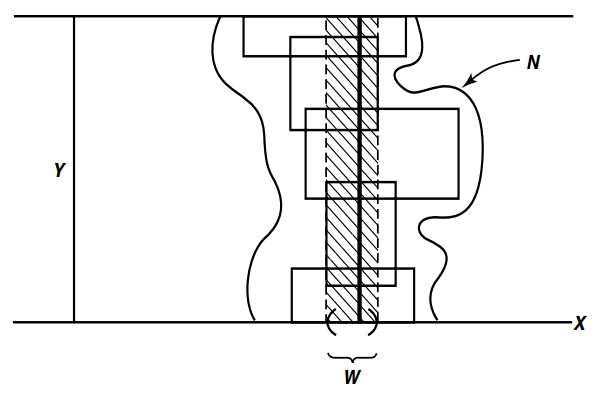
\includegraphics[scale = 0.45]{tube_slice_lemma.png}}
\end{minipage}
\caption{\footnotesize{\textbf{The tube of a slice $x_0 \times Y$ in neighborhood $N$ of product space. \citep{munkres2000topology}}}}
\label{fig: tube_slice_lemma}
\end{figure}

\begin{lemma} (\textbf{The Tube Lemma}).\citep{munkres2000topology} \\
Consider the product space $X \times Y$, where $Y$ is \textbf{compact}. If $N$ is an open set of $X \times Y$ containing the \textbf{slice} $x_0 \times Y$ of $X \times Y$, then $N$ contains some \textbf{tube} $W \times Y$ about $x_0 \times Y$, where $W$ is a \textbf{neighborhood} of $x_0$ in X.
\end{lemma}

\item \begin{remark}(\textbf{\emph{Compactness by Infinite Product}}) \\
Unlike \emph{the connectedness property}, which \emph{may not hold} for infinite product space, \emph{the infinite product of compact space is indeed compact}. This is called \emph{\textbf{the Tychonoff theorem}},
\end{remark}






\item To prove \emph{compactness}, the following property is useful:
\begin{definition} (\emph{\textbf{Finite Intersection Property}})\\
\emph{A collection $\srC$ of subsets} of $X$ is said to have \underline{\emph{\textbf{the finite intersection property}}} if for \emph{every finite subcollection}
\begin{align*}
\{C_1 \xdotx{,} C_n\}
\end{align*}
 of $\srC$, the \emph{\textbf{intersection}} $C_1 \xdotx{\cap} C_n$ is \emph{\textbf{nonempty}}.
\end{definition}

\item \begin{proposition} (\textbf{Equivalent Definition of Compactness}) \citep{munkres2000topology} \\
Let $X$ be a topological space. Then $X$ is \textbf{compact} \textbf{if and only if} for every collection $\srC$ of \textbf{closed} sets in $X$ having \textbf{the finite intersection property}, the intersection $\bigcap_{C\in \srC}C$ of all the elements of $\srC$ is \textbf{nonempty}.
\end{proposition}
\begin{proof}
Given a collection $\srA$ of subsets of $X$, let
\begin{align*}
\srC = \set{X \setminus A:  A \in \srA}
\end{align*}
be the collection of their \emph{complements}. Then the following statements hold:
\begin{enumerate}
\item $\srA$ is a collection of open sets if and only if $\srC$ is a collection of closed sets.
\item The collection $\srA$ covers $X$ if and only if the \emph{intersection} $\bigcap_{C \in \srC} C$ of all the elements of $\srC$ is \emph{\textbf{empty}}.
\item The \emph{\textbf{finite subcollection}} $\{A_1 \xdotx{,} A_n\}$ of $\srA$ covers $X$ if and only if the \emph{\textbf{intersection}} of the corresponding elements $C_i = X \setminus A_i$ of $\srC$ is \emph{\textbf{empty}}.
\end{enumerate}
The proof of the theorem now proceeds in two easy steps: taking the \emph{\textbf{contrapositive}} (of the theorem), and then the \emph{\textbf{complement}} (of the sets)!

There are two equivalent statements regarding the compactness of set:
\begin{enumerate}
\item ``\emph{Given any collection $\srA$ of open subsets of $X$, if $\srA$ covers $X$, then some finite subcollection of $\srA$ covers $X$.}"
\item ``\emph{Given any collection $\srA$ of open sets, if \textbf{no finite subcollection} of $\srA$ covers $X$, then $A$ \textbf{does not cover} $X$.}"

\item $\Rightarrow$  ``\emph{Given any collection $\srC$ of \textbf{closed sets}, if \textbf{every finite intersection} of elements of $\srC$ is \textbf{nonempty}, then the \textbf{intersection of all the elements} of $\srC$ is \textbf{nonempty}}" \qed
\end{enumerate}
\end{proof}



\item \begin{remark} (\emph{\textbf{Nested Sequence of Closed Sets in Compact Space}})\\
A special case of this proposition occurs when we have a \emph{\textbf{nested} sequence $C_1 \supseteq C_2 \xdotx{\supseteq} C_n \supseteq  \ldots$ of \textbf{closed sets}} in \emph{a \textbf{compact space} $X$}. 

If each of the sets $C_n$ is nonempty, then the collection $\srC = \set{C_n}_{n \in \bZ_{+}}$ automatically has \emph{\textbf{the finite intersection
property}}. Then the intersection
\begin{align*}
\bigcap_{n \in \bZ_{+}}C_n
\end{align*}
is nonempty.
\end{remark}
\end{itemize}
\subsection{Compact Subspaces of the Real Line}
\begin{itemize}
\item \begin{theorem}\citep{munkres2000topology}\\
Let $X$ be a \textbf{simply ordered} set having the \textbf{least upper bound property}. In the order topology, each \textbf{closed interval} in $X$ is \textbf{compact}.
\end{theorem}

\item \begin{corollary} (\textbf{Closed Interval in Real Line is Compact})\citep{munkres2000topology}\\
Every \textbf{closed interval} in $\bR$ is \textbf{compact}.
\end{corollary}

\item \begin{proposition}  (\textbf{Closed and Bounded in Euclidean Metric $=$ Compact})\citep{munkres2000topology}\\
A subspace $A$ of $\bR^n$ is \textbf{compact} if and only if it is \underline{\textbf{closed} and is \textbf{bounded}} in the \textbf{\underline{euclidean} metric} $d$ or the \textbf{square metric} $\rho$
\end{proposition}

\item \begin{theorem} (\textbf{Extreme Value Theorem}). \citep{munkres2000topology} \\
Let $f : X \rightarrow Y$ be \textbf{continuous}, where $Y$ is an \textbf{ordered set} in the order topology. If $X$ is \textbf{compact}, then there exist points $c$ and $d$ in $X$ such that $f(c) \le f(x) \le f (d)$ for every $x \in X$.
\end{theorem}

\item \begin{definition} (\emph{\textbf{Distance to Subset}})\\
Let $(X, d)$ be a \emph{\textbf{metric space}}; let $A$ be a nonempty subset of $X$. For each $x \in X$, we define \emph{\textbf{the distance} from $x$ to $A$} by the equation
\begin{align*}
d(x, A) = \inf\set{d(x, a): a \in A}.
\end{align*}
\end{definition}

\item \begin{remark}
The distance to subset $d(x: A)$ is a \emph{\textbf{continuous}} function with respect to the first argument.
\end{remark}


\item \begin{remark}
Recall that the \emph{\textbf{diameter}} of a \emph{bounded subset} $A$ of a \emph{metric space} $(X, d)$ is the number
\begin{align*}
\sup\set{d(a_1, a_2): a_1, a_2 \in A}.
\end{align*}
\end{remark}


\item \begin{lemma} (\textbf{The Lebesgue Number Lemma}). \citep{munkres2000topology} \\
Let $\srA$ be an \textbf{open covering} of the \textbf{metric space} $(X, d)$. If $X$ is \textbf{compact}, there is a $\delta > 0$ such that for each subset of $X$
having \textbf{diameter less than} $\delta$, there exists an element of $\srA$ containing it.

The number $\delta$ is called a \underline{\textbf{Lebesgue number}} for the covering $\srA$.
\end{lemma}

\item \begin{remark}
\emph{\textbf{The Lebesgue number}} is a \emph{\textbf{threshold} on \textbf{diameter of subset}} so that all of subsets with diameter less than this threshold is fully contained in one of the open sets in the covering of $X$. The \emph{existance} of this number relies on the \emph{\textbf{compactness}} of domain $X$.

This number is used in \emph{\textbf{$\epsilon$-$\delta$ condition}} to prove \emph{the uniform continuity}.
\end{remark}

\item \begin{definition} (\emph{\textbf{Uniform Continuity}})\\
A function $f: (X, d_X) \rightarrow (Y, d_Y)$ is said to be \underline{\emph{\textbf{uniformly continuous}}} if given $\epsilon > 0$, there is a $\delta > 0$ such that for every pair of points $x_0$, $x_1$ of $X$,
\begin{align*}
d_X(x_0, x_1) < \delta \quad \Rightarrow \quad d_Y(f(x_0), f(x_1)) < \epsilon. 
\end{align*}
\end{definition}

\item \begin{theorem} (\textbf{Uniform Continuity Theorem}). \citep{munkres2000topology} \\
 Let $f: X \rightarrow Y$ be a \textbf{continuous} map of the \textbf{compact} metric space $(X, d_X) $ to the metric space $(Y, d_Y)$. Then $f$ is \textbf{uniformly continuous}.
\end{theorem}
\begin{proof}
Given $\epsilon > 0$, take \emph{\textbf{the open covering}} of $Y$ by balls $B(y, \epsilon/2)$ of radius $\epsilon/2$. Let $\srA$ be \emph{\textbf{the open covering}} of $X$ by \emph{\textbf{the inverse images} of these balls under $f$}. Choose $\delta$ to be a \emph{\textbf{Lebesgue number}} for the covering $\srA$. Then if $x_1$ and $x_2$ are two points of $X$ such that $d_X(x_1, x_2) < \delta$, the two-point set $\set{x_1, x_2}$ has \emph{diameter less than $\delta$}, so that
its image $\set{f(x_1), f(x_2)}$ \emph{lies in some ball $B(y, \epsilon/2)$}. Then $d_Y(f(x_1), f(x_2)) < \epsilon$, as
desired.  \qed
\end{proof}

\item \begin{remark}
\begin{align*}
f\text{ continous } + \text{ compact domain } \Rightarrow f\text{ uniformly continous }
\end{align*}
\end{remark}

\item \begin{definition}
If $X$ is a space, a point $x$ of X is said to be \emph{\textbf{an isolated point}} of $X$ if \emph{the one-point set} $\{x\}$ is \emph{\textbf{open}} in $X$.
\end{definition}

\item \begin{theorem} (\textbf{Uncountability in Compact Hausdorff Space}) \citep{munkres2000topology}\\
Let $X$ be a nonempty \textbf{compact Hausdorff} space. If $X$ has \textbf{no isolated points}, then $X$ is \textbf{uncountable}.
\end{theorem}


\item \begin{corollary} \citep{munkres2000topology}\\
Every \textbf{closed interval} in $\bR$ is \textbf{uncountable}.
\end{corollary}

\item \begin{exercise} (\textbf{Cantor Set}) \citep{munkres2000topology}\\
Let $A_0$ be the \textbf{closed interval} $[0, 1]$ in $\bR$. Let $A_1$ be the set obtained from $A_0$ by \textbf{deleting} its ``\textbf{middle third}” $(1/3, 2/3)$. Let $A_2$ be the set obtained from $A_1$ by deleting its``middle thirds” $(1/9, 2/9)$ and $(7/9, 8/9)$. In general, define $A_n$ by the equation
\begin{align*}
A_n = A_{n-1} \setminus \paren{\bigcup_{k=0}^{\infty}\paren{\frac{1 + 3k}{3^k}, \frac{2 + 3k}{3^k}}}.
\end{align*}
The \textbf{intersection}
\begin{align*}
C = \bigcap_{n \in \bZ_{+}}A_n
\end{align*}
is called \underline{\textbf{the Cantor set}}; it is a \textbf{subspace} of $[0, 1]$.
\begin{enumerate}
\item Show that $C$ is \textbf{totally disconnected}.
\item Show that $C$ is \textbf{compact}.
\item Show that each set $A_n$ is a \textbf{union} of \textbf{finitely} many disjoint \textbf{closed intervals} of
length $1/3^n$; and show that the \textbf{end points} of these intervals lie in $C$.
\item Show that $C$ has \textbf{no isolated points}.
\item Conclude that $C$ is \textbf{uncountable}.
\end{enumerate}
\end{exercise}

\end{itemize}
\subsection{Limit Point Compactness}
\begin{itemize}
\item \begin{definition} (\emph{\textbf{Limit Point Compactness}})\\
A space $X$ is said to be \underline{\emph{\textbf{limit point compact}}} if \emph\textbf{{every infinite subset}} of $X$ has a \emph{\textbf{limit point}}.
\end{definition}

\item \begin{proposition}(\textbf{Compactness $\Rightarrow$ Limit Point Compactness}) \citep{munkres2000topology}\\
\textbf{Compactness} implies \textbf{limit point compactness}, but \textbf{not conversely}.
\end{proposition}

\item \begin{example}(\textbf{\emph{Limit Point Compactness $\not\Rightarrow$ Compactness}}) \\
Let $Y$ consist of \emph{\textbf{two points}}; give $Y$ the topology consisting of $Y$ and the empty set. Then the space $X = \bZ_{+} \times Y$ is \textbf{\emph{limit point compact}}, for \emph{every nonempty subset of $X$ has a \textbf{limit point}}. It is \emph{\textbf{not compact}}, for the \emph{covering} of $X$ by the open sets $U_n = \set{n} \times Y$ has \emph{no finite subcollection covering} $X$. \qed
\end{example}

\item \begin{definition} (\emph{\textbf{Sequential Compactness}})\\
Let $X$ be a topological space. If $(x_n)$ is a \emph{sequence} of points of $X$, and if
\begin{align*}
n_1 < n_2 < \ldots < n_i < \ldots
\end{align*}
is an increasing sequence of positive integers, then the sequence $(y_i)$ defined by setting $y_i = x_{n_i}$ is called a \emph{\textbf{subsequence}} of the sequence $(x_n)$. 

The space $X$ is said to be \underline{\emph{\textbf{sequentially compact}}} if \emph{every sequence of points of $X$ has a \textbf{convergent subsequence}}.
\end{definition}

\item \begin{theorem} (\textbf{Equivalent Definitions of Compactness in Metric Space}) \citep{munkres2000topology}\\
Let $X$ be a \textbf{metrizable space}. Then the following are \textbf{equivalent}:
\begin{enumerate}
\item $X$ is \textbf{compact}.
\item $X$ is \textbf{limit point compact}.
\item $X$ is \textbf{sequentially compact}.
\end{enumerate}
\end{theorem}
\end{itemize}
\subsection{Local Compactness}
\begin{itemize} 
\item \begin{definition} (\emph{\textbf{Local Compactness}})\\
A space $X$ is said to be \underline{\emph{\textbf{locally compact at $x$}}} if there is some \emph{\textbf{compact subspace}} $C$ of $X$ that contains a \emph{\textbf{neighborhood}} of $x$. 

If $X$ is \emph{locally compact} at \emph{each of its points}, $X$ is said simply to be \underline{\emph{\textbf{locally compact}}}.
\end{definition}

\item \begin{example} 
For the one-dimensional space:
\begin{enumerate}
\item The real line $\bR$ is \emph{\textbf{locally compact}}. The point $x$ lies in some interval $(a, b)$, which in turn is \emph{contained} in \emph{the compact subspace} $[a, b]$. 
\item The subspace $\bQ$ of rational numbers is \emph{\textbf{not locally compact}}.
\end{enumerate}
\end{example}


\item \begin{example}
For product space of $\bR$:
\begin{enumerate}
\item The \emph{\textbf{finite dimensional space}} $\bR^n$ is \emph{\textbf{locally compact}}; the point $x$ lies in some basis element
$(a_1, b_1) \xdotx{\times} (a_n, b_n)$, which in turn lies in \emph{the compact subspace} $[a_1, b_1] \xdotx{\times} [a_n, b_n]$.
\item The \emph{\textbf{countable infinite dimensional space}} $\bR^{\omega}$ is \emph{\textbf{not locally compact}}; \emph{none of its basis elements are contained in compact
subspaces.} For if
\begin{align*}
B = (a_1, b_1) \xdotx{\times} (a_n, b_n) \times \bR \xdotx{\times} \bR \times \ldots
\end{align*}
were contained in a \emph{compact subspace}, then its \emph{\textbf{closure}}
\begin{align*}
\bar{B} = [a_1, b_1] \xdotx{\times} [a_n, b_n] \times \bR \xdotx{\times} \bR \times \ldots
\end{align*}
would be \emph{\textbf{compact}}, which it is not.
\end{enumerate} 
\end{example}

\item \begin{example} (\emph{\textbf{Simply Ordered Set with Least Upper Bound Property}})\\
Every \underline{\emph{\textbf{simply ordered} set}} $X$ \emph{having \underline{\textbf{the least upper bound property}}} is \emph{\textbf{locally compact}}: Given a basis element for $X$, it is contained in a \emph{closed interval} in $X$, which is compact.
\end{example}

\item \begin{example} (\emph{\textbf{Manifold}}) \citep{lee2018introduction} \\
Every \underline{\emph{\textbf{topological manifold}}} is \emph{\textbf{locally compact Hausdorff}}.

Thus \underline{\emph{\textbf{every smooth manifold}}} is  \emph{\textbf{locally compact Hausdorff}}.
\end{example}


\item \begin{definition} (\emph{\textbf{Precompactness}})\\
A subset of $X$ is said to be \underline{\emph{\textbf{precompact}}} in $X$ if its \emph{\textbf{closure}} in $X$ is \emph{\textbf{compact}}.
\end{definition}

\item If $X$ is \emph{not a compact Hausdorff space}, then \emph{under what conditions} is $X$ \emph{homeomorphic} with \emph{a \textbf{subspace} of a compact Hausdorff space} ?

\begin{theorem} (\textbf{Unique One-Point Compactification}) \citep{munkres2000topology}\\
Let $X$ be a space. Then $X$ is \underline{\textbf{locally compact Hausdorff}} if and only if there exists a space $Y$ satisfying the following conditions:
\begin{enumerate}
\item $X$ is a subspace of $Y$.
\item The set $Y \setminus X$ consists of \textbf{a single point} (which is the limit point of $X$).
\item $Y$ is a \textbf{compact Hausdorff} space.
\end{enumerate} 
If $Y$ and $Y'$ are two spaces satisfying these conditions, then there is a \textbf{homeomorphism} of $Y$ with $Y'$ that equals \textbf{the identity map} on $X$.
\end{theorem}

\item \begin{definition} (\emph{\textbf{One-Point Compactification}})\\
If $Y$ is a \emph{\textbf{compact Hausdorff}} space and $X$ is a proper \emph{subspace} of $Y$ whose \emph{\textbf{closure}} equals $Y$, then $Y$ is said to be a \underline{\textbf{\emph{compactification}}} of $X$. 

If $Y\setminus X$ equals \emph{a single point}, then $Y$ is called \underline{\textbf{\emph{the one-point compactification}}} of $X$.
\end{definition}

\item \begin{remark} (\emph{\textbf{Locally Compact Hausdorff} $=$ Existance of Unique One-Point Compactification})\\
$X$ has a \emph{\textbf{one-point compactification}} $Y$ if and only if $X$ is a \emph{\textbf{locally compact Hausdorff space}} that is \emph{not itself compact}. 

We speak of $Y$ as ``\emph{\textbf{the}}" \emph{one-point compactification} because $Y$ is \emph{\textbf{uniquely}} determined up to a \emph{homeomorphism}.
\end{remark}

\item \begin{example}
\emph{\textbf{The one-point compactification}} of the real line $\bR$ is \emph{\textbf{homeomorphic}} with the \emph{\textbf{circle}} $\bS^1$.

Similarly, \emph{\textbf{the one-point compactification}} of $\bR^2$ is \emph{\textbf{homeomorphic}} to the \emph{\textbf{sphere}} $\bS^2$.
\end{example}

\item \begin{proposition} (\textbf{Locally Compact Hausdorff $=$ Precompact Basis}) \citep{munkres2000topology} \\
Let $X$ be a \textbf{Hausdorff} space. Then $X$ is \textbf{locally compact} \textbf{if and only if} given $x$ in $X$, and given a neighborhood $U$ of $x$, there is a neighborhood $V$ of $x$ such that $\bar{V}$ is \textbf{compact} and $\bar{V} \subseteq U$.
\end{proposition}

\item \begin{corollary} (\textbf{Closed or Open Subspace}) \citep{munkres2000topology} \\
Let $X$ be locally compact Hausdorff; let $A$ be a subspace of $X$. If $A$ is \textbf{closed} in $X$ or \textbf{open} in $X$, then $A$ is locally compact.
\end{corollary}

\item \begin{corollary}  \citep{munkres2000topology} \\
A space $X$ is \textbf{homeomorphic} to an \textbf{open} subspace of a \textbf{compact Hausdorff} space \textbf{if and only if} $X$ is \textbf{locally compact Hausdorff}.
\end{corollary}

\item \begin{remark}
\emph{Locally Compact Hausdorff $=$ Open Subspace of Compact Hausorff}
 \end{remark}

 \item \begin{theorem} \citep{treves2016topological}\\
 Every locally compact Hausdorff topological vector space is \textbf{finite-dimensional}.
 \end{theorem}

\item \begin{remark} (\textbf{\emph{Equivalent Definition of Locally Compact Hausdorff Space}})\\
For a \textbf{\emph{Hausdorff space}} $X$,  the following are \textbf{\emph{equivalent}}:
\begin{enumerate}
\item $X$ is \textbf{\emph{locally compact}}.
\item Each point of $X$ has a \textbf{\emph{precompact}} neighborhood. 
\item $X$ has a basis of \textbf{\emph{precompact}} open subsets.
\end{enumerate}
\end{remark}
\end{itemize}




\section{Nets and Convergence in Topological Space}
\begin{itemize}
\item \begin{definition} (\emph{\textbf{Directed System of Index Set}})\\
A \underline{\emph{\textbf{directed system}}} is \emph{an index set} $I$ together with an \emph{\textbf{ordering}} $\prec$ which satisfies:
\begin{enumerate}
\item If $\alpha, \beta \in l$ then there exists $\gamma \in I$ so that $\gamma \succ \alpha$ and $\gamma \succ \beta$.
\item $\prec$  is a \textbf{\emph{partial ordering}}.
\end{enumerate}
\end{definition}

\item \begin{definition}
A subset $K$ of $I$ is said to be \underline{\emph{\textbf{cofinal}}} in $I$ if for each $\alpha \in I$, there exists $\beta \in K$ such that $\alpha \preceq \beta$. 
\end{definition}

\item \begin{proposition}
If $I$ is a directed system, and $K$ is cofinal in $I$, then $K$ is a directed system. 
\end{proposition}

\item \begin{definition} (\textbf{\emph{Net}})\\
A \underline{\emph{\textbf{net}}} in a topological space $X$ is a mapping from a \emph{\textbf{directed system}} $I$ to $X$; we denote it by $\set{x_\alpha}_{\alpha \in I}$
\end{definition}

\item \begin{remark} (\emph{\textbf{Net} vs. \textbf{Sequence}})\\
\emph{\textbf{Net}} is a generalization and abstraction of \emph{\textbf{sequence}}. The directed system $I$ is \emph{\textbf{not necessarily countable}}. So $\set{x_\alpha}_{\alpha \in I}$ may not be a countable sequence. \emph{A sequence is a net with countable index set $I \subseteq \bN$}. The directed system can be any set e.g. a graph.
\end{remark}

\item \begin{definition}
If $P(\alpha)$ is a \emph{\textbf{proposition}} depending on an \emph{\textbf{index}} $\alpha$ in a \emph{directed set} $I$ we say \underline{\emph{\textbf{$P(\alpha)$ is eventually true}}} if there is a $\beta$ in $I$ with $P(\alpha)$ \emph{true} if \emph{for all} $\alpha \succ \beta$. 

We say \underline{\emph{\textbf{$P(\alpha)$ is frequently true}}} if it is \emph{\textbf{not eventually false}}, that is, if for any $\beta$ \emph{there exists} an $\alpha \succ \beta$ with $P(\alpha)$ \emph{true}.
\end{definition}

\item \begin{definition} (\emph{\textbf{Convergence}})\\
A \emph{\textbf{net}} $\set{x_\alpha}_{\alpha \in I}$  in a topological space $X$ is said to \underline{\emph{\textbf{converge}}} to a point $x \in X$ (written $x_{\alpha} \rightarrow x$) if for \textbf{\emph{any neighborhood}} $N$ of $x$, \emph{\textbf{there exists}} a $\beta \in l$ so that $x_{\alpha} \in N$ if $\alpha \succeq \beta$. The point $x$ that being converged to is called \underline{\emph{\textbf{the limit point}}} of  $x_{\alpha}$.

Note that if $x_\alpha \rightarrow x$, then $x_{\alpha}$ is \emph{\textbf{\underline{eventually} in all neighborhoods of}} $x$. If $x_{\alpha}$ is \emph{\textbf{\underline{frequently} in any neighborhood of}} $x$, we say that $x$ is a \underline{\emph{\textbf{cluster point}}} of $x_{\alpha}$. 
\end{definition}


\item \begin{remark}
This definition \emph{generalizes} the $\epsilon$-$\delta$ language for convergence in metric space.  Notice that the notions of \emph{limit} and \emph{cluster point} generalize the same notions for sequences in a metric space..
\end{remark} 

\item \begin{proposition} (\textbf{Net Lemma}) \citep{reed1980methods}\\
Let $A$ be a set in a topological space $X$. Then, a point $x \in \bar{A}$, the \textbf{closure} of $A$ \textbf{if and only if} there is a net $\set{x_\alpha}_{\alpha \in I}$ with $x_{\alpha} \in A$, So that $x_{\alpha} \rightarrow x$.
\end{proposition}

\item \begin{proposition} \citep{munkres2000topology}
\begin{enumerate}
\item (\textbf{Continuous Function}): A function $f$ from a topological space $X$ to a topological space $Y$ is \textbf{continuous} if and only if for \textbf{every convergent net} $\set{x_\alpha}_{\alpha \in I}$ \textbf{in $X$}, with $x_{\alpha} \rightarrow x$, the net $\{f(x_{\alpha})\}_{\alpha \in I}$ \textbf{converges in $Y$} to $f(x)$.
\item (\textbf{Uniqueness of Limit Point for Hausdorff Space}): Let $X$ be a \textbf{Hausdorff space}. Then a net $\set{x_\alpha}_{\alpha \in I}$ in $X$ can have \textbf{at most one limit}; that is, if $x_{\alpha} \rightarrow x$ and $x_{\alpha} \rightarrow y$, then $x = y$.
\end{enumerate}
\end{proposition}

\item \begin{definition}
A net  $\set{x_\alpha}_{\alpha \in I}$ is a \underline{\emph{\textbf{subnet}}} of a net  $\set{y_\beta}_{\beta \in J}$ if and only if there is
a function $F: I \rightarrow J$ such that
\begin{enumerate}
\item $x_\alpha = y_{F(\alpha)}$ for each $\alpha \in I$.
\item For all $\beta' \in J$, there is an $\alpha' \in I$ such that $\alpha \succ \alpha'$ implies $F(\alpha) \succ \beta'$ (that is,
$F(\alpha)$ is \emph{\textbf{eventually} \textbf{larger} than \textbf{any fixed}} $\beta \in J$ $\Rightarrow$ \underline{$F(I)$ is \textbf{\emph{cofinal}} in $J$}).
\end{enumerate}
\end{definition}

\item \begin{proposition}
A point $x$ in a topological space $X$ is a \textbf{cluster point} of a \textbf{net} $\set{x_\alpha}_{\alpha \in I}$ if and only if \textbf{some subnet} of $\set{x_\alpha}_{\alpha \in I}$ \textbf{converges} to $x$.
\end{proposition}

\item \begin{theorem} (\textbf{The Bolzano-Weierstrass Theorem}) \citep{reed1980methods, munkres2000topology} \\
A space $X$ is \textbf{compact} \textbf{if and only if} \textbf{every net} in $X$ \textbf{has a convergent subnet}.
\end{theorem}
\begin{proof}To prove the implication $\Rightarrow$, let $B_{\alpha} = \set{x_{\beta}: \alpha \preceq \beta}$ and show that
$\{B_{\alpha}\}$ has \emph{\textbf{the finite intersection property}}. 

To prove $\Leftarrow$, let $\srA$ be a collection of
\emph{\textbf{closed sets}} having \emph{the finite intersection property}, and let $\srB$ be the collection of
\emph{all finite intersections} of elements of $\srA$, \emph{\textbf{partially ordered}} by \emph{reverse inclusion}.
\end{proof}

\item \begin{remark} (\emph{\textbf{Compactness} via \textbf{Generalized Sequential Compactness}})\\
By \emph{generalization} of \emph{\textbf{squences}} $\Rightarrow$ \emph{\textbf{nets}}, we obtain a  \emph{generalization} of the result of \emph{\textbf{sequential compactnesss} in \textbf{metric space}} to \emph{\textbf{compactness}} in \emph{general topological space}.

With \emph{\textbf{first countable property}}, we can use subsequence and sequence in place of subnet and net.
\end{remark}
\end{itemize}
\newpage
\bibliographystyle{plainnat}
\bibliography{book_reference.bib}
\end{document}